\documentclass[12pt]{extarticle}
\usepackage{Format}
%\usepackage[draft]{graphicx}           % Uncomment and comment ``graphicx'' for decreasing compiling speeds
\usepackage{graphicx}


% First Page Header/footer
\fancypagestyle{firstpage}{
\lhead{ Dan Card\\                                     % Name
        Aerospace 523: Computational Fluid Dynamics I \\  % Class number and name
        Homework: 1                                    % Homework assignment
        \vspace{1cm}}
\rhead{ {\textit{dcard@umich.edu}}\\                   % Email
        \vspace{0.35cm}
        {Due: September 11\textsuperscript{th}, 2020}       % Due Date
        \vspace{1cm}}
\chead{}
\renewcommand{\headrulewidth}{3pt}}

% Header/Footer for the rest of the page
\pagestyle{fancy}{
\fancyhf{}
\lhead{Dan Card}                                                       % Name
\rhead{September 11, 2020}                                              % Due Date
\chead{\textit{Aerospace 523: Computational Fluid Dynamics I}}           % Class Name
\fancyfoot[l]{\textbf{University of Michigan - Ann Arbor}}             % University
\fancyfoot[r]{Page \thepage}}                                          % Page Number

\begin{document}      

        % Adjust Margins for first page
        \thispagestyle{firstpage}
        \newgeometry{left = 0.55in, right = 0.55in, top = 0in, bottom = 2.4in}
        \headsep = 65pt % Important! This creates a space between the header and the frame

        % Import problems .tex files
        \import{q1/}{q1.tex}     
        \import{q2/}{q2.tex}
        \import{q3/}{q3.tex}
        \import{q4/}{q4.tex}

        % Code attachments
        \pagebreak
        \section*{Python Code for Gram-Schmidt Orthonormalization}
        \lstinputlisting[
                linewidth=0.95\textwidth,
                xleftmargin=.1\textwidth,
                language=python,
                label=l:findb,
                caption={Gram-Schmidt Orthonormalization algorithm implementation in Python environment.}
                ]{q2/q2.py}

        \pagebreak
        \section*{Python Code for Newton-Raphson Method}
        \lstinputlisting[
                linewidth=0.95\textwidth,
                xleftmargin=.1\textwidth,
                language=python,
                label=l:findb,
                caption={Newton-Raphson algorithm implementation in Python environment.}
                ]{q3/q3.py}

        \pagebreak
        \section*{Matlab Code for Edge Connectivity}
        \lstinputlisting[
                linewidth=0.95\textwidth,
                xleftmargin=.1\textwidth,
                language=matlab,
                label=l:findb,
                caption={Edge Connectivity algorithm implementation in Matlab environment.}
                ]{q4/aero523_hw1_q4.m}

                \textcolor{white}{a}

                \pagebreak

                \section*{Matlab Command Window Output}
                \begin{figure}[h]
                        \centering
                        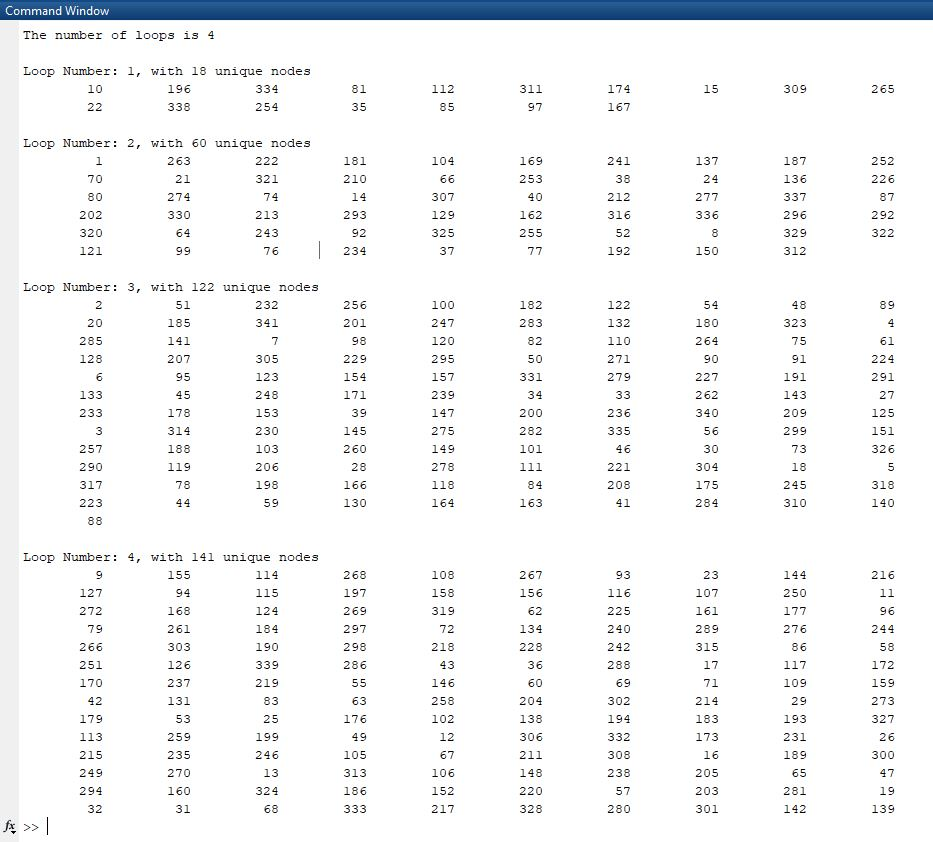
\includegraphics[width = 0.9\linewidth]{q4/q4_matlab_output.JPG}
                        \caption{Matlab Command Window output for tabulated node values.}
                        \label{fig:q4_matlab_output}
                \end{figure}
                
\end{document}


% Important formatting fixes for page layout

% Adjust Margins/Header/Footer for rest of homework (Add to page two)
        %\pagebreak
        %\pagestyle{fancy}
        %\restoregeometry

% Indent sections
        %\begin{adjustwidth}{2.5em}{0pt}
        %\end{adjustwidth}

% Input code used
        %\lstinputlisting[
        %linewidth=0.95\textwidth,
        %xleftmargin=.1\textwidth,
        %language=matlab,
        %label=l:findb,
        %caption={The caption}
        %]{aero523_hw4.m}